\subsubsection{Ausrichtung Drehturm}
\begin{figure}[h!]
	\centering
	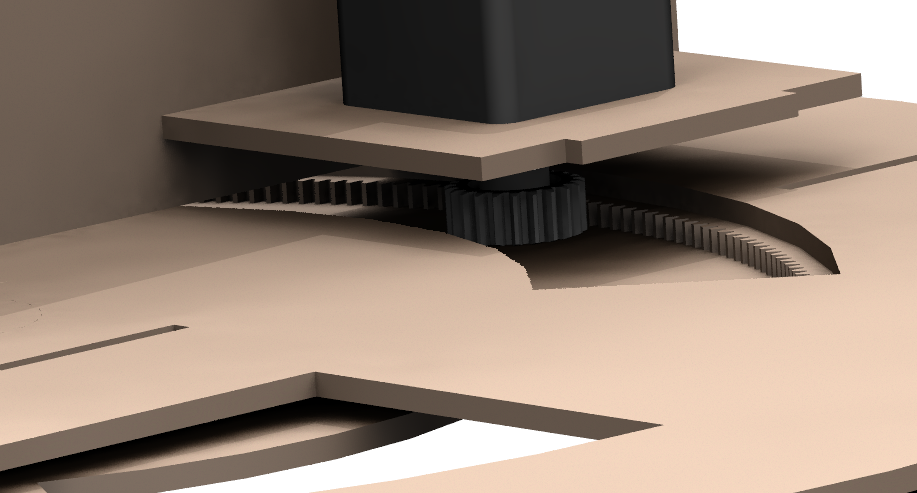
\includegraphics[width=\linewidth]{../../fig/Drehmechanismus}
	\caption{Drehmechanismus}
	\label{fig:Drehmechanismus}
\end{figure}
\paragraph{Komponentenbeschrieb}

Die horizontale Ausrichtung der Maschine auf den Korb, wird mittels einem Schrittmotor ermöglicht. An der Hauptachse des Motors ist ein Kunststoff-Zahnrad angebracht, welches in eine gebogene Zahnstange eingreift und somit durch Rotation eine Drehung des Drehturmes bewirkt. Die Zahnstange ist auf der Grundplatte befestigt, welche fix auf dem Tisch liegt. Auf dieser Grundplatte ist eine weitere, auf einem im Mittelpunkt der Grundplatte gelagerten Zapfen, rotierbare Platte angebracht. Die zwei Platten, sowie die Zahnstange wurden über NX konstruiert und mit einer Laserschneidmaschine aus MDF gefertigt.

\paragraph{Entwicklungsprozess}

Gemäss Aufgabenstellung sollten sich nach Abschluss des Wurfvorganges fünf Bälle im Korb befinden. Da die Position des Korbes nicht fix vorgegeben ist, würde ein einfaches befördern der Bälle nach vorne nicht ausreichen. Um die Wurfvorrichtung ausrichten zu können, musste daher ein weiterer Aktor her. Grundsätzlich wären ein seitliches Verschieben der kompletten Maschine, oder eine Eigenrotation in Frage gekommen. Da eine seitliche Verschiebung in vielerlei Hinsicht schwieriger auszuführen wäre, entschied man sich für die Eigenrotation.